% !TEX encoding = UTF-8 Unicode
% !TEX TS-program = xelatex
\begin{QUESTIONS}
    \begin{QUESTION}
        \begin{ExamInfo}{106}{學測}{單選}{1}
        \end{ExamInfo}
        \begin{ExamAnsRateInfo}{53}{82}{52}{25}
        \end{ExamAnsRateInfo}
        \begin{QBODY}
            已知某校老師玩過「寶可夢」的比率為${{r}_{1}}$,而學生玩過的比率為${{r}_{2}}$,其中${{r}_{1}}\ne {{r}_{2}}$。
            由下列選項中的資訊,請選出可以判定全校師生玩過「寶可夢」的比率之選項。
            \begin{QOPS}
                \QOP 全校老師與學生比率     
                \QOP 全校老師人數
                \QOP 全校學生人數
                \QOP 全校師生人數
                \QOP 全校師生玩過「寶可夢」人數
            \end{QOPS}
        \end{QBODY}
        \begin{QFROMS}
        \end{QFROMS}
        \begin{QTAGS}\QTAG{平均數}\QTAG{B2C4-1一維數據分析}\QTAG{B2C4數據分析}\end{QTAGS}
        \begin{QANS}
            (1)
        \end{QANS}
        \begin{QSOLLIST}
            \begin{QSOL}
                設老師人數:學生人數為 $m:n$\\
                則全校師生玩過寶可夢的比例為:$\FR{m r_1 + n r_2}{m+n} = \FR{m}{m+n} r_1 +\FR{n}{m+n} r_2$\\
                若是得到師生人數比例即可求全校師生玩過寶可夢的比率。
            \end{QSOL}
        \end{QSOLLIST}
        \begin{QEMPTYSPACE}
        \end{QEMPTYSPACE}
    \end{QUESTION}
    \begin{QUESTION}
        \begin{ExamInfo}{106}{學測}{單選}{2}
        \end{ExamInfo}
        \begin{ExamAnsRateInfo}{51}{84}{52}{17}
        \end{ExamAnsRateInfo}
        \begin{QBODY}
            某個手機程式,每次點擊螢幕上的數$a$後,螢幕上的數會變成${{a}^{2}}$。當一開始時螢幕上的數$b$為正且連續點擊螢幕三次後,螢幕上的數接近${{81}^{3}}$。試問實數$b$最接近下列哪一個選項?
			\begin{QOPS}
				\QOP $1.7$      
				\QOP $3$      
				\QOP $5.2$      
				\QOP $9$      
				\QOP $81$
			\end{QOPS}
        \end{QBODY}
        \begin{QFROMS}
        \end{QFROMS}
        \begin{QTAGS}\QTAG{B1C3-1指數}\QTAG{B1C3指對數函數}\QTAG{指數律}\end{QTAGS}
        \begin{QANS}
            (3)
        \end{QANS}
        \begin{QSOLLIST}
            \begin{QSOL}
                由題意可得 $(((b)^2)^2)^2 = b^8 = 81^3 \Rightarrow b^8 = 3^12 \Rightarrow b=3^{\FR{12}{8}} = 3^{\FR{3}{2}} = \sqrt{27} $ \\
                由 $5=\sqrt{25}$ 可估計得 $b \approx 5.3$ \\
                故選 (3)
            \end{QSOL}
        \end{QSOLLIST}
        \begin{QEMPTYSPACE}
        \end{QEMPTYSPACE}
    \end{QUESTION}
    \begin{QUESTION}
        \begin{ExamInfo}{106}{學測}{單選}{3}
        \end{ExamInfo}
        \begin{ExamAnsRateInfo}{38}{71}{34}{9}
        \end{ExamAnsRateInfo}
        \begin{QBODY}
            設$\Gamma :\frac{{{y}^{2}}}{{{a}^{2}}}-\frac{{{x}^{2}}}{{{b}^{2}}}=1$為坐標平面上一雙曲線,且其通過第一象限的漸近線為$\ell $。考慮動點$(t,{{t}^{2}})$,從時間$t=0$時出發。當$t>0$時,請選出正確的選項。(題意補充 $a>0,b>0$)
			\begin{QOPS}
			\QOP 此動點不會碰到$\Gamma $,也不會碰到$\ell $
			\QOP 此動點會碰到$\Gamma $,但不會碰到$\ell $
			\QOP 此動點會碰到$\ell $,但不會碰到$\Gamma $
			\QOP 此動點會先碰到$\Gamma $,再碰到$\ell $
			\QOP 此動點會先碰到$\ell $,再碰到$\Gamma $
			\end{QOPS}
        \end{QBODY}
        \begin{QFROMS}
        \end{QFROMS}
        \begin{QTAGS}\QTAG{B4C4-3雙曲線}\QTAG{B4C4二次曲線}\QTAG{圖形}\end{QTAGS}
        \begin{QANS}
            (5)
        \end{QANS}
        \begin{QSOLLIST}
            \begin{QSOL}
                \begin{QSTEPS}
                    \QSTEP{$\Gamma :\frac{{{y}^{2}}}{{{a}^{2}}}-\frac{{{x}^{2}}}{{{b}^{2}}}=1$為一個上下型、中心在原點的雙曲線 }
                    \QSTEP{動點 $(t,{{t}^{2}}), t>0$ 的圖形為 $y=x^2, x>0$ 的拋物線右半部}
                    \QSTEP{作圖如下:%TODO:詳解圖
                    }
                    \QSTEP{故選(5)}
                \end{QSTEPS}
            \end{QSOL}
        \end{QSOLLIST}
        \begin{QEMPTYSPACE}
        \end{QEMPTYSPACE}
    \end{QUESTION}
    \begin{QUESTION}
        \begin{ExamInfo}{106}{學測}{單選}{4}
        \end{ExamInfo}
        \begin{ExamAnsRateInfo}{55}{89}{60}{16}
        \end{ExamAnsRateInfo}
        \begin{QBODY}
            在右下圖的正立方體上有兩質點分別自頂點$A,C$同時出發,各自以等速直線運動分別向頂點$B,D$前進,且在1秒後分別同時到達$B,D$。請選出這段時間兩質點距離關係的正確選項。
        
			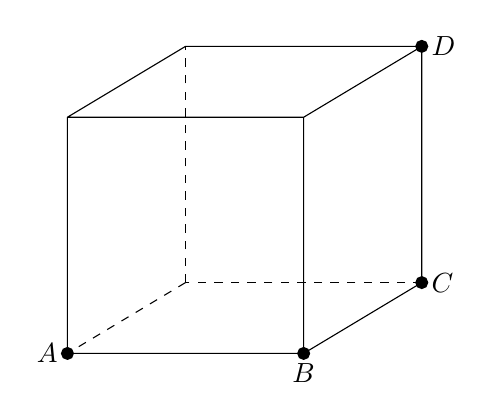
\begin{tikzpicture}[every edge quotes/.append style={auto, text=blue},
			x={(-0.25cm,-0.15cm)},
			y={(0.5cm,0cm)},
			z={(0cm,0.5cm)}]
			%%空間坐標中的CUBE 是以平面上的x軸 y軸再去擴充出深度z軸 z 往前為正,向後為負
			\coordinate (O) at (0,0,0);
			\coordinate (x) at (7,0,0);
			\coordinate (y) at 
			(0,7,0);
			\coordinate (z) at (0,0,7);
			
			\coordinate (Base1) at (0,0,0);
			\coordinate (Base2) at (6,0,0);
			\coordinate (Base3) at (6,6,0);
			\coordinate (Base4) at (0,6,0);
			\coordinate (Base1Up) at (0,0,6);
			\coordinate (Base2Up) at (6,0,6);
			\coordinate (Base3Up) at (6,6,6);
			\coordinate (Base4Up) at (0,6,6);
			
			\coordinate (A) at (Base2);
			\coordinate (B) at (Base3);
			\coordinate (C) at (Base4);
			\coordinate (D) at (Base4Up);
			
			\draw [draw=black, every edge/.append style={draw=black, dashed}]
			(Base1) edge (Base2)
			(Base2) -- (Base3)
			(Base3) -- (Base4)
			(Base4) edge (Base1)
			(Base1Up) -- (Base2Up)
			(Base2Up) -- (Base3Up)
			(Base3Up) -- (Base4Up)
			(Base4Up) -- (Base1Up)
			(Base1) edge (Base1Up)
			(Base2) -- (Base2Up)
			(Base3) -- (Base3Up)
			(Base4) -- (Base4Up);
			
			\foreach \v/\u/\t in 
			{ A/left/$A$,
				B/below/$B$,
				C/right/$C$,
				D/right/$D$
			}
			{
				\draw[ultra thick,fill] (\v) circle (1.5pt);
				\node[\u] at (\v){\t};
			}; 
			
			\end{tikzpicture}
			
			\begin{QOPS}
				\QOP 兩質點的距離固定不變
				\QOP 兩質點的距離越來越小
				\QOP 兩質點的距離越來越大
				\QOP 在$\frac{1}{2}$秒時兩質點的距離最小
				\QOP 在$\frac{1}{2}$秒時兩質點的距離最大
			\end{QOPS}
        \end{QBODY}
        \begin{QFROMS}
        \end{QFROMS}
        \begin{QTAGS}\QTAG{B4C1-2空間向量的坐標表示法}\QTAG{B4C1空間向量}\end{QTAGS}
        \begin{QANS}
            (4)
        \end{QANS}
        \begin{QSOLLIST}
            \begin{QSOL}
                \begin{QSTEPS}
                    %TODO:圖
                    \QSTEP{建立坐標系可得 $A(1,0,0), B(1,1,0), C(0,1,0), D(0,1,1)$}
                    \QSTEP{令開始移動 $t$秒後\\
                           由$A$到$B$的質點動點坐標為$(1,t,0)$\\
                           由$C$到$D$的質點動點坐標為$(0,1,t)$}
                    \QSTEP{此兩質點的距離 \\
                        $\begin{aligned}
                        d &= \sqrt{1^2 + (t-1)^2+(0-t)^2} \\
                          &= \sqrt{2t^2-2t+2}\\
                          &= \sqrt{2(t-\frac{1}{2})^2 + \frac{3}{2}}
                        \end{aligned} $\\
                        根號內為$t$的二次式
                        當 $t=\frac{1}{2}$ 時,有最小值,故選(4)
                         }
                \end{QSTEPS}
            \end{QSOL}
        \end{QSOLLIST}
        \begin{QEMPTYSPACE}
        \end{QEMPTYSPACE}
    \end{QUESTION}
    \begin{QUESTION}
        \begin{ExamInfo}{106}{學測}{單選}{5}
        \end{ExamInfo}
        \begin{ExamAnsRateInfo}{37}{64}{35}{12}
        \end{ExamAnsRateInfo}
        \begin{QBODY}
            下圖是某城市在2016年的各月最低溫(橫軸$x$)與最高溫(縱軸$y$)的散佈圖。
            今以溫差(最高溫減最低溫)為橫軸且最高溫為縱軸重新繪製一散佈圖。試依此選出正確的選項。
            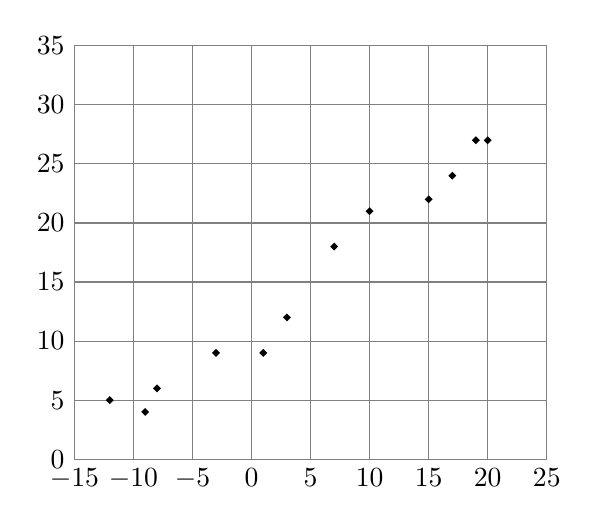
\begin{tikzpicture}[scale=0.15]
            \draw[color=gray, step=5] (-15,0) grid (25,35);
            \foreach \myy/\myx in 
            {
                5/-12,
                4/-9,
                6/-8,
                9/-3,
                9/1,
                12/3,
                18/7,
                21/10,
                22/15,
                24/17,
                27/19,
                27/20
            }
            {
                \draw[ultra thick,fill] (\myx,\myy) circle (2pt);
                
            };	    
            \foreach \itemx in {-15,-10,-5,...,25}
            {
                \node[below] at (\itemx, 0){$\scriptsize \itemx$};
            }
            
            \foreach \itemy in {0,5,10,...,35}
            {
                \node[left] at (-15,\itemy){$\scriptsize \itemy$};
            }
            
            \end{tikzpicture}
            
			\begin{QOPS}
				\QOP 最高溫與溫差為正相關,且它們的相關性比最高溫與最低溫的相關性強
				\QOP 最高溫與溫差為正相關,且它們的相關性比最高溫與最低溫的相關性弱
				\QOP 最高溫與溫差為負相關,且它們的相關性比最高溫與最低溫的相關性強
				\QOP 最高溫與溫差為負相關,且它們的相關性比最高溫與最低溫的相關性弱
				\QOP 最高溫與溫差為零相關
			\end{QOPS}
        \end{QBODY}
        \begin{QFROMS}
        \end{QFROMS}
        \begin{QTAGS}\QTAG{B2C4-2二維數據分析}\QTAG{圖表判讀}\QTAG{B2C4數據分析}\QTAG{相關係數}\end{QTAGS}
        \begin{QANS}
            (4)
        \end{QANS}
        \begin{QSOLLIST}
            \begin{QSOL}
                今以溫差(最高溫減最低溫)為橫軸且最高溫為縱軸重新繪製一散佈圖如下:
                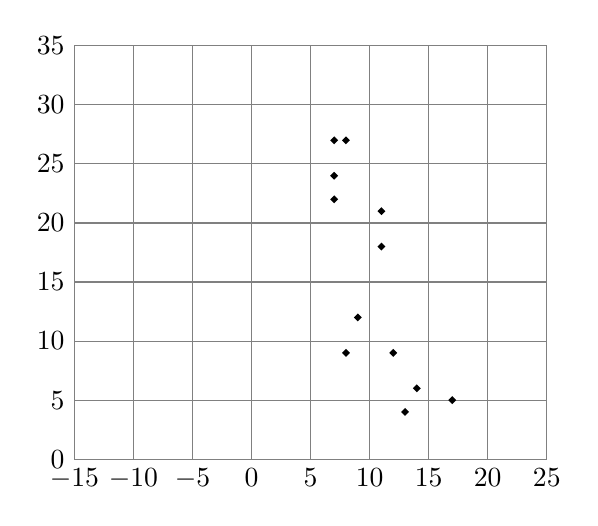
\begin{tikzpicture}[scale=0.15]
                    \draw[color=gray, step=5] (-15,0) grid (25,35);
                    \foreach \myy/\myx in 
                    {
                        5/-12,
                        4/-9,
                        6/-8,
                        9/-3,
                        9/1,
                        12/3,
                        18/7,
                        21/10,
                        22/15,
                        24/17,
                        27/19,
                        27/20
                    }
                    {
                        \draw[ultra thick,fill] (\myy-\myx,\myy) circle (2pt);
                        
                    };	    
                    \foreach \itemx in {-15,-10,-5,...,25}
                    {
                        \node[below] at (\itemx, 0){$\scriptsize \itemx$};
                    }
                    
                    \foreach \itemy in {0,5,10,...,35}
                    {
                        \node[left] at (-15,\itemy){$\scriptsize \itemy$};
                    }
                \end{tikzpicture}
                
                由散佈圖判斷可得:負相關,相關性比起原題目中的散布圖較弱。
            \end{QSOL}
        
            \begin{QSOL}
                在原圖上標示溫差的直線方程式$y-x=k$,$k=5,10,15,20$如下圖,\\
                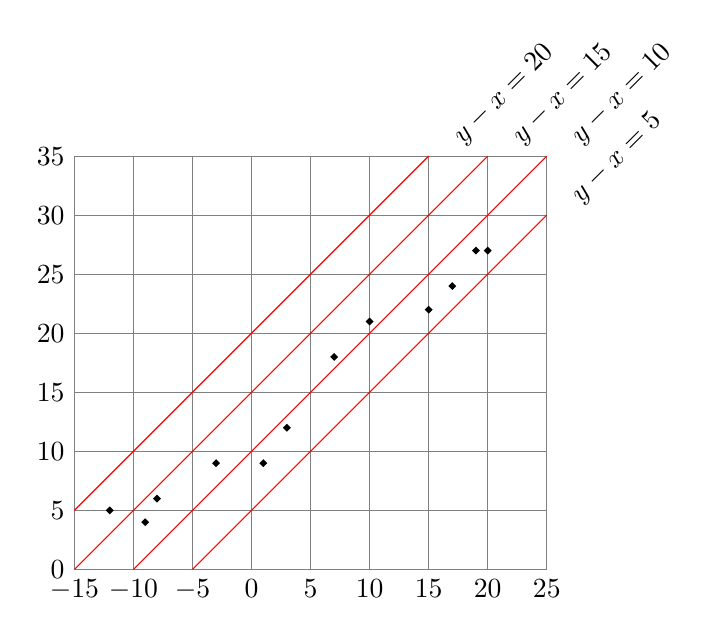
\begin{tikzpicture}[scale=0.15]
                    \draw[color=gray, step=5] (-15,0) grid (25,35);
                    \foreach \myy/\myx in 
                    {
                        5/-12,
                        4/-9,
                        6/-8,
                        9/-3,
                        9/1,
                        12/3,
                        18/7,
                        21/10,
                        22/15,
                        24/17,
                        27/19,
                        27/20
                    }
                    {
                        \draw[ultra thick,fill] (\myx,\myy) circle (2pt);
                        
                    };	    
                    \foreach \itemx in {-15,-10,-5,...,25}
                    {
                        \node[below] at (\itemx, 0){$\scriptsize \itemx$};
                    };
                    
                    \foreach \itemy in {0,5,10,...,35}
                    {
                        \node[left] at (-15,\itemy){$\scriptsize \itemy$};
                    };
                    
                    \foreach \startx/\starty/\endx/\endy/\myword in 
                    {-15/5/15/35/$y-x=20$,
                        -15/0/20/35/$y-x=15$,
                        -10/0/25/35/$y-x=10$,
                        -5/0/25/30/$y-x=5$
                    }
                    {    
                        \draw[color=red] (\startx,\starty) -- (\endx,\endy);
                        \node[label={[label distance=0.2cm,text depth=0ex,rotate=45]right:\myword}] at (\endx,\endy) {};
                    }
                \end{tikzpicture}
                
                注意其$y$ 坐標與 $y-x$值得對應關係,\\
                其集中分散程度較原本的散佈圖弱,且當 $y$ 坐標越大,$y-x$對應值越小,為負相關
                \\
                故選(4)
                
            \end{QSOL}
        
            \begin{QSOL}
                觀察原圖的相關係數,相當接近$1$,迴歸直線約為$y=0.7x$
                經過線性變換後 $r(y-x,y)\approx r(-0.3x,0.7x) <0$ 應為負相關\\
                利用 $0.7x$來估算 $y$ ,再次疊代誤差應會過大,故相關性較原有相關性弱。選 (4)
            \end{QSOL}
        \end{QSOLLIST}
        \begin{QEMPTYSPACE}
        \end{QEMPTYSPACE}
    \end{QUESTION}
    \begin{QUESTION}
        \begin{ExamInfo}{106}{學測}{單選}{6}
        \end{ExamInfo}
        \begin{ExamAnsRateInfo}{22}{43}{16}{7}
        \end{ExamAnsRateInfo}
        \begin{QBODY}
            試問有多少個實數$x$滿足$\frac{\pi }{2}\le x\le \frac{3\pi }{2}$且$\cos x{}^\circ \le \cos x$?
			\begin{QOPS}
				\QOP $0$個     
				\QOP $1$個     
				\QOP $2$個     
				\QOP $4$個     
				\QOP 無窮多個
			\end{QOPS}
        \end{QBODY}
        \begin{QFROMS}
        \end{QFROMS}
        \begin{QTAGS}\QTAG{B3C1三角}\QTAG{B3C1-2廣義角與極坐標}\end{QTAGS}
        \begin{QANS}
            (1)
        \end{QANS}
        \begin{QSOLLIST}
            \begin{QOP}
                \begin{QSTEPS}
                    \QSTEP{注意$\cos x{}^\circ \le \cos x$左右兩側一個使用度度量的三角函數,一個使用弳度量的三角函數}
                    \QSTEP{$\frac{\pi }{2}\le x\le \frac{3\pi }{2} \Rightarrow (\frac{\pi }{2})^\circ \le x^\circ \le (\frac{3\pi }{2})^\circ \Rightarrow 1\circ\le x^\circ \le 5^\circ\Rightarrow  \cos x^\circ > 0$}
                    \QSTEP{$ \frac{\pi }{2}\le x\le \frac{3\pi }{2} \Rightarrow \cos x \le 0$}
                    \QSTEP{$\cos x{}^\circ \le \cos x$ 左側恆正,右側負或$0$,故$x$ 為 $0$個實數解}
                \end{QSTEPS}
            \end{QOP}
        \end{QSOLLIST}
        \begin{QEMPTYSPACE}
        \end{QEMPTYSPACE}
    \end{QUESTION}
    \begin{QUESTION}
        \begin{ExamInfo}{106}{學測}{單選}{7}
        \end{ExamInfo}
        \begin{ExamAnsRateInfo}{29}{40}{27}{20}
        \end{ExamAnsRateInfo}
        \begin{QBODY}
            小明想要安排從星期一到星期五共五天的午餐計畫。他的餐點共有四種選擇:牛肉麵、大滷麵、咖哩飯及排骨飯。小明想要依據下列兩原則來安排他的午餐:
			(甲)每天只選一種餐點但這五天中每一種餐點至少各點一次
			(乙)連續兩天的餐點不能重複且不連續兩天吃麵食
			根據上述原則,小明這五天共有幾種不同的午餐計畫?
			\begin{QOPS}
				\QOP $52$      
				\QOP $60$      
				\QOP $68$      
				\QOP $76$      
				\QOP $84$
			\end{QOPS}
        \end{QBODY}
        \begin{QFROMS}
        \end{QFROMS}
        \begin{QTAGS}\QTAG{B2C2-2排列}\QTAG{乘法原理加法原理}\QTAG{B2C2-1簡單的邏輯與集合}\QTAG{B2C2排列組合}\QTAG{重複排列}\end{QTAGS}
        \begin{QANS}
            (2)
        \end{QANS}
        \begin{QSOLLIST}
            \begin{QSOL}
                \begin{QSTEPS}
                    \QSTEP{共有五天,卻只有四種餐點,必定有一種餐點吃兩天,其餘各吃一天。\\
                        令牛肉麵、大滷麵、咖哩飯及排骨飯分別為$A,B,C,D$, 方法數討論如下:                    
                        \begin{SOLCASES}
                            \SOLCASE{$A$餐兩天:麵食類為 $AAB$ 可排列,但其間隔處必排$CD$(可排列)\\以滿足麵食不得相鄰的條件 \\
                            方法數:$\FR{3!}{2!} \times 2! = 6$}
                            \SOLCASE{$B$餐兩天:麵食類為 $ABB$ 方法同 $A$ 餐兩天
                                方法數:$\FR{3!}{2!} \times 2!=6$}
                            \SOLCASE{$C$餐兩天:麵食類為$AB$,飯食類為$CCD$,可先取全部排列後,扣除$AB$相鄰與$CC$相鄰\\
                                全部 $-$ ($AB$相鄰)$\cup$ ($CC$ 相鄰) \\
                                $=\FR{5!}{2!} - \FR{4!}{2!}\time 2! - 4! + 3!\times 2!$\\
                                $= 24$
                            }
                            \SOLCASE{$D$餐兩天:麵食類為$AB$,飯食類為$CDD$,計算方式與$C$餐兩天同\\
                                方法數$24$
                            }
                        \end{SOLCASES}                    
                    }
                    \QSTEP{合計:$6+6+24+24=60$}
                \end{QSTEPS}
            \end{QSOL}
        \end{QSOLLIST}
        \begin{QEMPTYSPACE}
        \end{QEMPTYSPACE}
    \end{QUESTION}
\end{QUESTIONS}
\begin{QUESTIONS}
    \begin{QUESTION}
        \begin{ExamInfo}{106}{學測}{多選}{8}
        \end{ExamInfo}
        \begin{ExamAnsRateInfo}{24}{35}{20}{17}
        \end{ExamAnsRateInfo}
        \begin{QBODY}
            設$m,n$為小於或等於$4$的相異正整數且$a,b$為非零實數。已知函數$f(x)=a{{x}^{m}}$與函數$g(x)=b{{x}^{n}}$的圖形恰有$3$個相異交點,請選出可能的選項。
			\begin{QOPS}
			\QOP $m,n$皆為偶數且$a,b$同號 
			\QOP $m,n$皆為偶數且$a,b$異號
			\QOP $m,n$皆為奇數且$a,b$同號
			\QOP $m,n$皆為奇數且$a,b$異號
			\QOP $m,n$為一奇一偶
			\end{QOPS}
        \end{QBODY}
        \begin{QFROMS}
        \end{QFROMS}
        \begin{QTAGS}\QTAG{B1C2多項式函數}\QTAG{B1C2-1簡單的多項式及圖形}\QTAG{單項函數圖形}\end{QTAGS}
        \begin{QANS}
            (1)(3)
        \end{QANS}
        \begin{QSOLLIST}
            \begin{QSOL}
                %依選項討論逐一畫圖
            \end{QSOL}
            \begin{QSOL}
                \begin{QSTEPS}
                    \QSTEP{在不失一般性的條件下,令 $m>=n$}
                    \QSTEP{兩個函數的圖形交點,即為方程組 $\left\lbrace\begin{array}{l}  
                        y=f(x)=ax^m\\
                        y=g(x)=bx^n
                        \end{array}\right.$ 的解\\
                    兩式相減可得 $ax^m-bx^n = 0 \Rightarrow x^n(ax^{m-n}-b)=0 \Rightarrow x =0 或 x^{m-n}=\FR{b}{a}$\\}
                    \QSTEP{已知函數$f(x)=a{{x}^{m}}$與函數$g(x)=b{{x}^{n}}$的圖形恰有$3$個相異交點,表示方程組有$3$組相異實根 $\Rightarrow x^{m-n}=\FR{b}{a}$有兩個相異實根 }
                    \QSTEP{由 $m-n \in \left\lbrace0,1,2,3 \right\rbrace$考慮以下四個單項函數圖形,僅有$m-n=2$ 與 $a,b$同號才有兩個相異實根,故選(1)(3)
                    %TODO:補圖,單項函數 x^0,~ x^3 的圖形
                 }
                \end{QSTEPS}
            \end{QSOL}
        \end{QSOLLIST}
        \begin{QEMPTYSPACE}
        \end{QEMPTYSPACE}
    \end{QUESTION}
    \begin{QUESTION}
        \begin{ExamInfo}{106}{學測}{多選}{9}
        \end{ExamInfo}
        \begin{ExamAnsRateInfo}{34}{57}{30}{15}
        \end{ExamAnsRateInfo}
        \begin{QBODY}
            設$\Gamma $為坐標平面上的圓,點$(0,0)$在$\Gamma $的外部且點$(2,6)$在$\Gamma $的內部。請選出正確的選項。
			\begin{QOPS}
			\QOP $\Gamma $的圓心不可能在第二象限
			\QOP $\Gamma $的圓心可能在第三象限且此時$\Gamma $的半徑必定大於10
			\QOP $\Gamma $的圓心可能在第一象限且此時$\Gamma $的半徑必定小於10
			\QOP $\Gamma $的圓心可能在$x$軸上且此時圓心的$x$坐標必定小於10
			\QOP $\Gamma $的圓心可能在第四象限且此時$\Gamma $的半徑必定大於10
			\end{QOPS}
        \end{QBODY}
        \begin{QFROMS}
        \end{QFROMS}
        \begin{QTAGS}\QTAG{B3C2-3圓與直線的關係}\QTAG{B3C2直線與圓}\end{QTAGS}
        \begin{QANS}
            (5)
        \end{QANS}
        \begin{QSOLLIST}
            \begin{QSOL}
                \begin{QSTEPS}
                    \QSTEP{設圓心 $C(x,y), O(0,0), A(2,6)$}
                    \QSTEP{$O$在圓的內部,$A$ 在圓的外部 $\Rightarrow \overline{CO} >\overline{CA}$\\
                    $\Rightarrow \sqrt{x^2+y^2} > \sqrt{(x-2)^2 + (y-6)^2} \Rightarrow 0>-4x-12y+40\\ \Rightarrow x+3y>10$
                    則圓心落在此半平面上 %TODO:畫半平面的圖形
                    }
                    \QSTEP{如圖,計算出$x+3y=10$與$x$軸交點與$y$軸交點,判斷得(5)正確。}
                \end{QSTEPS}
            \end{QSOL}            
        \end{QSOLLIST}
        \begin{QEMPTYSPACE}
        \end{QEMPTYSPACE}
    \end{QUESTION}
    \begin{QUESTION}
        \begin{ExamInfo}{106}{學測}{多選}{10}
        \end{ExamInfo}
        \begin{ExamAnsRateInfo}{43}{66}{39}{24}
        \end{ExamAnsRateInfo}
        \begin{QBODY}
            坐標空間中有三直線${{L}_{1}}:\dfrac{x-1}{2}=\dfrac{y+1}{2}=\dfrac{z}{1},{{L}_{2}}:\left\{ \begin{aligned}
			& x-2y+2z=-4 \\ 
			& x+y-4z=5 \\ 
			\end{aligned} \right.,{{L}_{3}}:\left\{ \begin{aligned}
			& x=-t \\ 
			& y=-2-t \\ 
			& z=4+4t \\ 
			\end{aligned} \right.$,$t$為實數。請選出正確的選項。
			\begin{QOPS}
				\QOP ${{L}_{1}}$與${{L}_{2}}$的方向向量互相垂直
				\QOP ${{L}_{1}}$與${{L}_{3}}$的方向向量互相垂直
				\QOP 有一個平面同時包含${{L}_{1}}$與${{L}_{2}}$
				\QOP 有一個平面同時包含${{L}_{1}}$與${{L}_{3}}$
				\QOP 有一個平面同時包含${{L}_{2}}$與${{L}_{3}}$
			\end{QOPS}
        \end{QBODY}
        \begin{QFROMS}
        \end{QFROMS}
        \begin{QTAGS}\QTAG{B4C2-2空間直線方程式}\QTAG{兩線關係}\QTAG{B4C2空間中的平面與直線}\QTAG{面線關係}\QTAG{參數式}\end{QTAGS}
        \begin{QANS}
            (2)(3)(4)
        \end{QANS}
        \begin{QSOLLIST}
            \begin{QSOL}
                觀察題目所給的 $L_1,L_2,L_3$ 盡可能找出其通過的點以及方向向量\\
                $L_1:$ 方向向量可取為 $\lvec{v_1} = (2,2,1)$ ,過點 $P_1:(1,-1,0)$\\
                $L_2:$ 方向向量可取為 $\lvec{v_2} = (1,-2,2)\times(1,1,-4)=(6,6,3)$\\
                $L_3:$ 方向向量可取為 $\lvec{v_3} = (-1,-1, 4)$,過點 $P_3:(0,-2,4)$\\
                
                兩直線關係共有:重合、平行、交一點、歪斜。\\
                若是兩直線重合、平行、交一點,則有一平面同時包含兩直線。\\
                若是兩直線歪斜,則沒有一平面同時包含此兩直線。\\
                \begin{QOPSSOLLIST}
                    \QOPSSOL{$\lvec{v_1} \cdot \lvec{v_2} = (2,2,1) \cdot (6,6,3) \ne 0 \Rightarrow $ ${{L}_{1}}$與${{L}_{2}}$的方向向量沒有垂直,該選項錯誤。 }
                    \QOPSSOL{$\lvec{v_1} \cdot \lvec{v_3} = (2,2,1) \cdot (-1,-1,4) = 0 \Rightarrow $
                    ${{L}_{1}}$與${{L}_{3}}$的方向向量互相垂直,該選項正確。}
                    \QOPSSOL{因為 $\lvec{v_1} \parallel \lvec{v_2} \Rightarrow {L_1} \parallel {L_2} $或兩直線重合 $\Rightarrow$  有一個平面同時包含${{L}_{1}}$與${{L}_{2}}$,該選項正確。}
                    \QOPSSOL{因為 ${{L}_{1}}$與${{L}_{3}}$的方向向量互相垂直,尚須確認 $L_1$ 與$L_3$ 是相交一點還是歪斜。
                            將 $L_3$ 之參數式代入 $L_1$ 可得 $\FR{-t-1}{2} = \FR{-2-t+1}{2} = \FR{4+4t}{1}$ 可解得 $t = -1$,恰一組解\\
                            $L_1$ 與 $L_3$ 為相交一點,有一個平面同時包含${{L}_{1}}$與${{L}_{3}}$,該選項正確。}
                    \QOPSSOL{因為 ${{L}_{2}}$與${{L}_{3}}$的方向向量互相垂直,尚須確認 $L_2$ 與$L_3$ 是相交一點還是歪斜 \\
                            將 $L_3$ 之參數式代入 $L_2$ 可得 $\left\lbrace\begin{array}{l}  
                                                                            -t+4+2t+8+8t=-4  \\
                                                                            -t-2-t-16-16t=5  \\
                                                                            
                                                                        \end{array}\right.\Rightarrow \left\lbrace\begin{array}{l}  
                                                                           t=-\frac{16}{9}  \\
                                                                           t=-\frac{23}{18}  \\
                                                                        \end{array}\right.$ (兩個$t$值不同) $\Rightarrow L_2, L_3$ 歪斜 ,沒有一個平面同時包含${{L}_{2}}$與${{L}_{3}}$,該選項錯誤。
                                                            }
                \end{QOPSSOLLIST}
            \end{QSOL}
        \end{QSOLLIST}
        \begin{QEMPTYSPACE}
        \end{QEMPTYSPACE}
    \end{QUESTION}
    \begin{QUESTION}
        \begin{ExamInfo}{106}{學測}{多選}{11}
        \end{ExamInfo}
        \begin{ExamAnsRateInfo}{62}{84}{64}{38}
        \end{ExamAnsRateInfo}
        \begin{QBODY}
            設最近數學家發現一種新的可以無縫密舖平面的凸五邊形$ABCDE$,其示意圖如下。關於這五邊形,請選出正確的選項。
			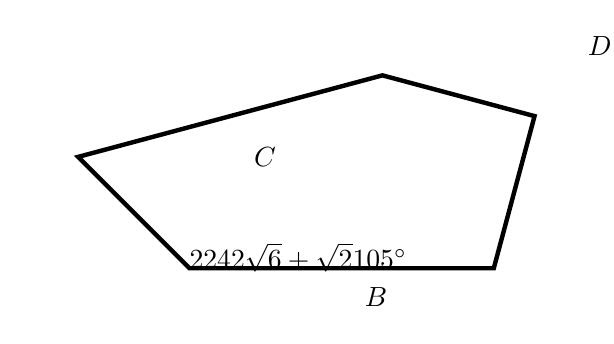
\begin{tikzpicture}[scale=1.0]
				\coordinate (B) at (0,0);
				\coordinate (A) at (0:{sqrt(6)+sqrt(2)});
				\path (A) ++(75:2) coordinate (E);
				\path (E) ++(165:2) coordinate (D);
				\coordinate (C) at (135:2);
				
				
				\draw[ultra thick] (A) -- (B)--(C)--(D)--(E) --cycle;
				\tkzLabelSegment[midway,  right](E,A){$2$};
				\tkzLabelSegment[midway,  above](D,E){$2$};
				\tkzLabelSegment[midway,  above](D,C){$4$};
				\tkzLabelSegment[midway,  below left](C,B){$2$};
				\tkzLabelSegment[midway,  below](B,A){$\sqrt{6}+\sqrt{2}$};
				\tkzMarkRightAngle[size=0.3](D,E,A);
				\tkzMarkAngle[size=0.3](E,A,B);
				\tkzLabelAngle[pos=0.6](E,A,B){$105^\circ$};
				
				\node[label=315:$A$] at (A){};
				\node[label=225:$B$] at (B){};
				\node[label=180:$C$] at (C){};
				\node[label=90:$D$] at (D){};
				\node[label=45:$E$] at (E){};
			\end{tikzpicture}
			\begin{QOPS}
    			\QOP $\overline{AD}=2\sqrt[{}]{2}$
    			\QOP $\angle DAB=45{}^\circ $
    			\QOP $\overline{BD}=2\sqrt[{}]{6}$
    			\QOP $\angle ABD=45{}^\circ $
    			\QOP $BCD$的面積為$2\sqrt[{}]{2}$
			\end{QOPS}
        \end{QBODY}
        \begin{QFROMS}
        \end{QFROMS}
        \begin{QTAGS}\QTAG{面積}\QTAG{B3C1-3正弦定理與餘弦定理}\QTAG{B3C1三角}\end{QTAGS}
        \begin{QANS}
            (1)(4)
        \end{QANS}
        \begin{QSOLLIST}
            \begin{QSOL}
                \begin{QOPSSOLLIST}
                    連接 $\overline{DA},\overline{DB}$
                    \QOPSSOL{ $\triangle ADE$ 為等腰直角三角形 ,又 $\overline{DE}=2 \Rightarrow \overline{AD} = 2\sqrt{2}$ }
                    \QOPSSOL{ $\angle DAB = \angle EAB - \angle EAD = 105^\circ - 45^\circ = 60^\circ $}
                    \QOPSSOL{ 在$\triangle ABD$ 中使用餘弦定理:\\
                                $\begin{aligned}
                                \overline{BD} & = \sqrt{\overline{AD}^2 + \overline{AB}^2 - 2\cdot \overline{AD} \cdot \overline{AB} \cos 60^\circ}\\
                                              & = \sqrt{(2\sqrt{2})^2 + (\sqrt{6} + \sqrt{2})^2 - 2 \cdot 2\sqrt{2} \cdot (\sqrt{6} + \sqrt{2})\cdot \frac{1}{2}}\\
                                              & =2\sqrt{3} 
                                \end{aligned}$
                             }
                    \QOPSSOL{在$\triangle ABD$ 中使用正弦定理:\\
                                $\FR{\overline{DB}}{\sin \angle DAB} = \FR{\overline{DA}}{\sin \angle DBA}
                                 \Rightarrow \FR{2\sqrt{3}}{\frac{\sqrt{3}}{2}} = \FR{2\sqrt{2}}{\sin \angle ABD} 
                                 \Rightarrow \sin \angle ABD = \FR{\sqrt{2}}{2}
                                 \Rightarrow \angle ABD = 45\circ \vee 135\circ$ (但 $135^\circ$ 顯然不合)}
                    \QOPSSOL{已知 $\triangle BCD$ 中三邊長為 $4,2,2\sqrt{3}$,為 $2:1:\sqrt{3}$ 之$30^\circ - 60^\circ -90^\circ$ 三角形\\
                             其面積為:$\frac{1}{2} \times 2 \times 2\sqrt{3} = 2\sqrt{3}$
                    }
                \end{QOPSSOLLIST}
                故選(1)(4)
            \end{QSOL}
        \end{QSOLLIST}
        \begin{QEMPTYSPACE}
        \end{QEMPTYSPACE}
    \end{QUESTION}
    \begin{QUESTION}
        \begin{ExamInfo}{106}{學測}{多選}{12}
        \end{ExamInfo}
        \begin{ExamAnsRateInfo}{28}{37}{27}{20}
        \end{ExamAnsRateInfo}
        \begin{QBODY}
            某班級50位學生,段考國文、英文、數學及格的人數分別為45、39、34人,且英文及格的學生國文也都及格。現假設數學和英文皆及格的有$x$人,數學及格但英文不及格的有$y$人。請選出正確的選項。
			\begin{QOPS}
				\QOP $x+y=39$
				\QOP $y\le 11$
				\QOP 三科中至少有一科不及格的學生有$39-x+y$人
				\QOP 三科中至少有一科不及格的學生最少有11人
				\QOP 三科中至少有一科不及格的學生最多有27人
			\end{QOPS}
        \end{QBODY}
        \begin{QFROMS}
        \end{QFROMS}
        \begin{QTAGS}\QTAG{集合}\QTAG{B2C2-1簡單的邏輯與集合}\QTAG{B2C2排列組合}\end{QTAGS}
        \begin{QANS}
            (2)(5)
        \end{QANS}
        \begin{QSOLLIST}
            \begin{QSOL}
				\begin{QSTEPS}
					\QSTEP{ 令全班為集合$U$,國文、數學、英文,及格的集合分別為 $C,M,E$ \\
							可得:$n(C) = 45, n(M) = 34 , n(E) = 39$}
					\QSTEP{ $x+y = n (M \cap E) + n (M \cap \overline{E}) = n(M) = 34$,則 (1) 錯誤}
					\QSTEP{ $n(\bar{E}) = 50 -39 =11 \ge n (M \cap \bar{E}) \Rightarrow y \le 11$,則 (2) 正確}
					\QSTEP{ 由以上兩步驟可得 $23 \le x\le 34$}
					\QSTEP{ 至少一科不及格 $= n(\text{全}) - n (C\cap M\cap E) = 50-x$,\\
							可得 $16 \le \text{至少一科不及格} \le 27$}
				\end{QSTEPS}
				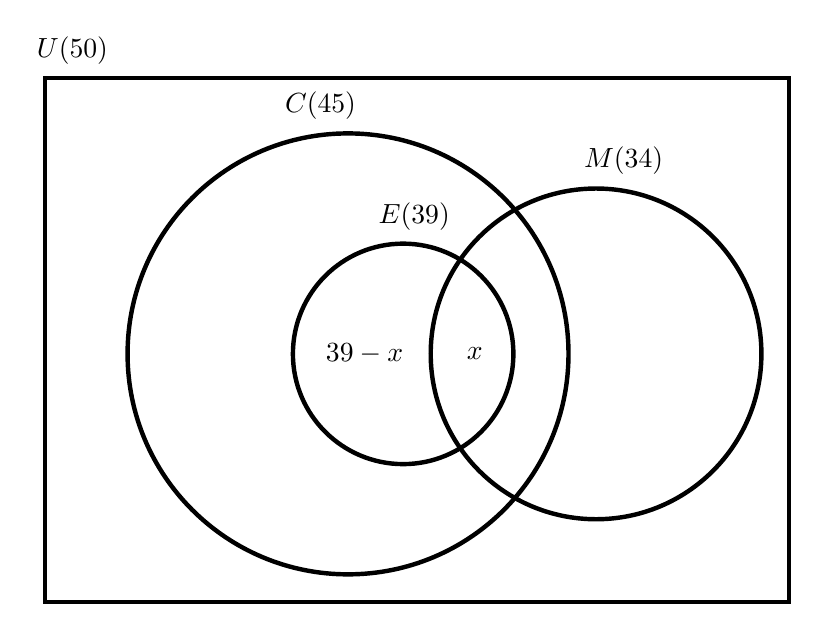
\begin{tikzpicture}[scale=0.7]
					\draw[ultra thick]  (-6.5,6) circle (2);
					\draw[ultra thick]  (-7.5,6) node (v1) {} ellipse (4 and 4);
					\draw[ultra thick]  (-3,6) node (v2) {} circle (3);
					\draw[ultra thick]  (-13,11) rectangle (0.5,1.5);
					\node at (-12.5,11.5) {$U(50)$};
					\node at (-8,10.5) {$C(45)$};
					\node at (-5.2,6) {$x$};
					\node at (-7.2,6) {$39-x$};
					\node at (-6.3,8.5) {$E(39)$};
					\node at (-2.5,9.5) {$M(34)$};
				\end{tikzpicture}
			\end{QSOL}

        \end{QSOLLIST}
        \begin{QEMPTYSPACE}
        \end{QEMPTYSPACE}
    \end{QUESTION}
    \begin{QUESTION}
        \begin{ExamInfo}{106}{學測}{多選}{13}
        \end{ExamInfo}
        \begin{ExamAnsRateInfo}{36}{54}{32}{22}
        \end{ExamAnsRateInfo}
        \begin{QBODY}
            空間中有一四面體$ABCD$。假設$\lvec{AD}$分別與$\lvec{AB}$和$\lvec{AC}$垂直,請選出正確的選項。
			\begin{QOPS}
				\QOP $\lvec{DB}\cdot\lvec{DC} ={{\overline{DA}}^{2}}- \lvec{AB}\cdot \lvec{AC}$
				\QOP 若$\angle BAC$是直角,則$\angle BDC$是直角
				\QOP 若$\angle BAC$是銳角,則$\angle BDC$是銳角
				\QOP 若$\angle BAC$是鈍角,則$\angle BDC$是鈍角
				\QOP 若$\overline{AB}<\overline{DA}$且$\overline{AC}<\overline{DA}$,則$\angle BDC$是銳角
			\end{QOPS}
        \end{QBODY}
        \begin{QFROMS}
        \end{QFROMS}
        \begin{QTAGS}\QTAG{B4C1-3空間向量的內積}\QTAG{B4C1空間向量}\end{QTAGS}
        \begin{QANS}
            (3)(5)
        \end{QANS}
        \begin{QSOLLIST}
        \end{QSOLLIST}
        \begin{QEMPTYSPACE}
        \end{QEMPTYSPACE}
    \end{QUESTION}
\end{QUESTIONS}
\begin{QUESTIONS}
    \begin{QUESTION}
        \begin{ExamInfo}{106}{學測}{填充}{A}
        \end{ExamInfo}
        \begin{ExamAnsRateInfo}{54}{82}{60}{20}
        \end{ExamAnsRateInfo}
        \begin{QBODY}
            遞迴數列$\langle {{a}_{n}}\rangle $滿足${{a}_{n}}={{a}_{n-1}}+f(n-2)$,其中$n\ge 2$且$f(x)$為二次多項式。若${{a}_{1}}=1,{{a}_{2}}=2,{{a}_{3}}=5,{{a}_{4}}=12$,則${{a}_{5}}= \TCNBOX{ \TCN\TCN }$     。
        \end{QBODY}
        \begin{QFROMS}
        \end{QFROMS}
        \begin{QTAGS}\QTAG{B2C1數列級數}\QTAG{遞迴}\QTAG{B2C1-1數列}\end{QTAGS}
        \begin{QANS}
            $25$
        \end{QANS}
        \begin{QSOLLIST}
        \end{QSOLLIST}
        \begin{QEMPTYSPACE}
        \end{QEMPTYSPACE}
    \end{QUESTION}
    \begin{QUESTION}
        \begin{ExamInfo}{106}{學測}{填充}{B}
        \end{ExamInfo}
        \begin{ExamAnsRateInfo}{26}{65}{12}{1}
        \end{ExamAnsRateInfo}
        \begin{QBODY}
            坐標平面上,$ABC$內有一點$P$滿足$\lvec{AP}=(\frac{4}{3},\frac{5}{6})$及$\lvec{AP}=\frac{1}{2}\lvec{AB}+\frac{1}{5}\lvec{AC}$。若$A,P$連線交$\overline{BC}$於$M$,則$\lvec{AM}= \TCNBOX{\left(\FR{\TCN\TCN}{\TCN\TCN} ,\FR{\TCN\TCN}{\TCN\TCN} \right)}$。(化成最簡分數)
        \end{QBODY}
        \begin{QFROMS}
        \end{QFROMS}
        \begin{QTAGS}\QTAG{線性組合}\QTAG{B3C3-1平面向量的表示法}\QTAG{B3C3平面向量}\end{QTAGS}
        \begin{QANS}
            $(\dfrac{40}{21},\dfrac{25}{21})$
        \end{QANS}
        \begin{QSOLLIST}
        \end{QSOLLIST}
        \begin{QEMPTYSPACE}
        \end{QEMPTYSPACE}
    \end{QUESTION}
    \begin{QUESTION}
        \begin{ExamInfo}{106}{學測}{填充}{C}
        \end{ExamInfo}
        \begin{ExamAnsRateInfo}{30}{63}{22}{5}
        \end{ExamAnsRateInfo}
        \begin{QBODY}
            若$a$為正整數且方程式$5{{x}^{3}}+(a+4){{x}^{2}}+ax+1=0$的根都是有理根,則$a= \TCNBOX{\TCN}$     。
        \end{QBODY}
        \begin{QFROMS}
        \end{QFROMS}
        \begin{QTAGS}\QTAG{B1C2-3多項式方程式}\QTAG{B1C2多項式函數}\QTAG{牛頓定理}\end{QTAGS}
        \begin{QANS}
            $7$
        \end{QANS}
        \begin{QSOLLIST}
        \end{QSOLLIST}
        \begin{QEMPTYSPACE}
        \end{QEMPTYSPACE}
    \end{QUESTION}
    \begin{QUESTION}
        \begin{ExamInfo}{106}{學測}{填充}{D}
        \end{ExamInfo}
        \begin{ExamAnsRateInfo}{37}{70}{33}{8}
        \end{ExamAnsRateInfo}
        \begin{QBODY}
            設${{a}_{1}},{{a}_{2}},\cdots ,{{a}_{9}}$為等差數列且$k$為實數。若方程組
			$\left\{ \begin{aligned}
			& {{a}_{1}}x-{{a}_{2}}y+2{{a}_{3}}z=k+1 \\ 
			& {{a}_{4}}x-{{a}_{5}}y+2{{a}_{6}}z=-k-5 \\ 
			& {{a}_{7}}x-{{a}_{8}}y+2{{a}_{9}}z=k+9 \\ 
			\end{aligned} \right.$有解,
			則$k=\TCNBOX{\TCN\TCN}$      。
        \end{QBODY}
        \begin{QFROMS}
        \end{QFROMS}
        \begin{QTAGS}\QTAG{B2C1數列級數}\QTAG{B4C3矩陣}\QTAG{B4C3-1線性方程組與矩陣}\QTAG{等差數列}\QTAG{方程組}\end{QTAGS}
        \begin{QANS}
            $-5$
        \end{QANS}
        \begin{QSOLLIST}
        \end{QSOLLIST}
        \begin{QEMPTYSPACE}
        \end{QEMPTYSPACE}
    \end{QUESTION}
    \begin{QUESTION}
        \begin{ExamInfo}{106}{學測}{填充}{E}
        \end{ExamInfo}
        \begin{ExamAnsRateInfo}{24}{59}{12}{1}
        \end{ExamAnsRateInfo}
        \begin{QBODY}
            設$a,b,x$皆為正整數且滿足$a\le x\le b$及$b-a=3$。若用內插法從$\log a,\log b$求得$\log x$的
			近似值為
			$\log x\approx \frac{1}{3}\log a+\frac{2}{3}\log b=\frac{1}{3}(1+2\log 3-\log 2)+\frac{2}{3}(4\log 2+\log 3)$,
			則$x$的值為 $\TCNBOX{\TCN\TCN}$        。
        \end{QBODY}
        \begin{QFROMS}
        \end{QFROMS}
        \begin{QTAGS}\QTAG{內插法}\QTAG{B1C3指對數函數}\QTAG{B1C3-5指數與對數的應用}\end{QTAGS}
        \begin{QANS}
            $47$
        \end{QANS}
        \begin{QSOLLIST}
        \end{QSOLLIST}
        \begin{QEMPTYSPACE}
        \end{QEMPTYSPACE}
    \end{QUESTION}
    \begin{QUESTION}
        \begin{ExamInfo}{106}{學測}{填充}{F}
        \end{ExamInfo}
        \begin{ExamAnsRateInfo}{19}{45}{11}{1}
        \end{ExamAnsRateInfo}
        \begin{QBODY}
            一隻青蛙位於坐標平面的原點,每步隨機朝上、下、左、右跳一單位長,總共跳了四步。青蛙跳了四步後恰回到原點的機率為$\TCNBOX{\FR{\TCN}{\TCN\TCN}}$。(化成最簡分數)
        \end{QBODY}
        \begin{QFROMS}
        \end{QFROMS}
        \begin{QTAGS}\QTAG{B2C3機率}\QTAG{B2C3-2機率的定義與性質}\end{QTAGS}
        \begin{QANS}
            $\dfrac{9}{64}$
        \end{QANS}
        \begin{QSOLLIST}
        \end{QSOLLIST}
        \begin{QEMPTYSPACE}
        \end{QEMPTYSPACE}
    \end{QUESTION}
    \begin{QUESTION}
        \begin{ExamInfo}{106}{學測}{填充}{G}
        \end{ExamInfo}
        \begin{ExamAnsRateInfo}{22}{56}{9}{1}
        \end{ExamAnsRateInfo}
        \begin{QBODY}
            地面上甲、乙兩人從同一地點同時開始移動。甲以每秒4公尺向東等速移動,乙以每秒3公尺向北等速移動。在移動不久之後,他們互望的視線被一圓柱體 建築物阻擋了6秒後才又相見。此圓柱體建築物底圓的直徑為$\TCNBOX{\TCN\TCN.\TCN}$公尺。
        \end{QBODY}
        \begin{QFROMS}
        \end{QFROMS}
        \begin{QTAGS}\QTAG{B3C2-3圓與直線的關係}\QTAG{B3C2-1直線方程式及其圖形}\QTAG{B3C2直線與圓}\end{QTAGS}
        \begin{QANS}
            $14.4$
        \end{QANS}
        \begin{QSOLLIST}
        \end{QSOLLIST}
        \begin{QEMPTYSPACE}
        \end{QEMPTYSPACE}
    \end{QUESTION}
\end{QUESTIONS}
